%!TeX encoding = UTF-8
%!TeX program = xelatex
\documentclass[notheorems, aspectratio=54]{beamer}
% aspectratio: 1610, 149, 54, 43(default), 32

\usepackage{latexsym}
\usepackage{amsmath,amssymb}
\usepackage{mathtools}
\usepackage{color,xcolor}
\usepackage{graphicx}
\usepackage{algorithm}
\usepackage{amsthm}
\usepackage{lmodern} % 解决 font warning
\usepackage[UTF8]{ctex}
\usepackage{animate} % insert gif

\usepackage{lipsum} % To generate test text 
\usepackage{ulem} % 下划线,波浪线

\usepackage{listings} % display code on slides; don't forget [fragile] option after \begin{frame}

% ----------------------------------------------
% tikx
\usepackage{framed}
\usepackage{tikz}
\usepackage{pgf}
\usetikzlibrary{calc,trees,positioning,arrows,chains,shapes.geometric,%
    decorations.pathreplacing,decorations.pathmorphing,shapes,%
    matrix,shapes.symbols}
\pgfmathsetseed{1} % To have predictable results
% Define a background layer, in which the parchment shape is drawn
\pgfdeclarelayer{background}
\pgfsetlayers{background,main}

% define styles for the normal border and the torn border
\tikzset{
  normal border/.style={orange!30!black!10, decorate, 
     decoration={random steps, segment length=2.5cm, amplitude=.7mm}},
  torn border/.style={orange!30!black!5, decorate, 
     decoration={random steps, segment length=.5cm, amplitude=1.7mm}}}

% Macro to draw the shape behind the text, when it fits completly in the
% page
\def\parchmentframe#1{
\tikz{
  \node[inner sep=2em] (A) {#1};  % Draw the text of the node
  \begin{pgfonlayer}{background}  % Draw the shape behind
  \fill[normal border] 
        (A.south east) -- (A.south west) -- 
        (A.north west) -- (A.north east) -- cycle;
  \end{pgfonlayer}}}

% Macro to draw the shape, when the text will continue in next page
\def\parchmentframetop#1{
\tikz{
  \node[inner sep=2em] (A) {#1};    % Draw the text of the node
  \begin{pgfonlayer}{background}    
  \fill[normal border]              % Draw the ``complete shape'' behind
        (A.south east) -- (A.south west) -- 
        (A.north west) -- (A.north east) -- cycle;
  \fill[torn border]                % Add the torn lower border
        ($(A.south east)-(0,.2)$) -- ($(A.south west)-(0,.2)$) -- 
        ($(A.south west)+(0,.2)$) -- ($(A.south east)+(0,.2)$) -- cycle;
  \end{pgfonlayer}}}

% Macro to draw the shape, when the text continues from previous page
\def\parchmentframebottom#1{
\tikz{
  \node[inner sep=2em] (A) {#1};   % Draw the text of the node
  \begin{pgfonlayer}{background}   
  \fill[normal border]             % Draw the ``complete shape'' behind
        (A.south east) -- (A.south west) -- 
        (A.north west) -- (A.north east) -- cycle;
  \fill[torn border]               % Add the torn upper border
        ($(A.north east)-(0,.2)$) -- ($(A.north west)-(0,.2)$) -- 
        ($(A.north west)+(0,.2)$) -- ($(A.north east)+(0,.2)$) -- cycle;
  \end{pgfonlayer}}}

% Macro to draw the shape, when both the text continues from previous page
% and it will continue in next page
\def\parchmentframemiddle#1{
\tikz{
  \node[inner sep=2em] (A) {#1};   % Draw the text of the node
  \begin{pgfonlayer}{background}   
  \fill[normal border]             % Draw the ``complete shape'' behind
        (A.south east) -- (A.south west) -- 
        (A.north west) -- (A.north east) -- cycle;
  \fill[torn border]               % Add the torn lower border
        ($(A.south east)-(0,.2)$) -- ($(A.south west)-(0,.2)$) -- 
        ($(A.south west)+(0,.2)$) -- ($(A.south east)+(0,.2)$) -- cycle;
  \fill[torn border]               % Add the torn upper border
        ($(A.north east)-(0,.2)$) -- ($(A.north west)-(0,.2)$) -- 
        ($(A.north west)+(0,.2)$) -- ($(A.north east)+(0,.2)$) -- cycle;
  \end{pgfonlayer}}}

% Define the environment which puts the frame
% In this case, the environment also accepts an argument with an optional
% title (which defaults to ``Example'', which is typeset in a box overlaid
% on the top border
\newenvironment{parchment}[1][Example]{%
  \def\FrameCommand{\parchmentframe}%
  \def\FirstFrameCommand{\parchmentframetop}%
  \def\LastFrameCommand{\parchmentframebottom}%
  \def\MidFrameCommand{\parchmentframemiddle}%
  \vskip\baselineskip
  \MakeFramed {\FrameRestore}
  \noindent\tikz\node[inner sep=1ex, draw=black!20,fill=white, 
          anchor=west, overlay] at (0em, 2em) {\sffamily#1};\par}%
{\endMakeFramed}

% ----------------------------------------------

\mode<presentation>{
    \usetheme{CambridgeUS}
    % Boadilla CambridgeUS
    % default Antibes Berlin Copenhagen
    % Madrid Montpelier Ilmenau Malmoe
    % Berkeley Singapore Warsaw
    \usecolortheme{beaver}
    % beetle, beaver, orchid, whale, dolphin
    \useoutertheme{infolines}
    % infolines miniframes shadow sidebar smoothbars smoothtree split tree
    \useinnertheme{circles}
    % circles, rectanges, rounded, inmargin
}
% 设置 block 颜色
\setbeamercolor{block title}{bg=red!30,fg=white}

\newcommand{\reditem}[1]{\setbeamercolor{item}{fg=red}\item #1}

% 缩放公式大小
\newcommand*{\Scale}[2][4]{\scalebox{#1}{\ensuremath{#2}}}

% 解决 font warning
\renewcommand\textbullet{\ensuremath{\bullet}}

% ---------------------------------------------------------------------
% flow chart
\tikzset{
    >=stealth',
    punktchain/.style={
        rectangle, 
        rounded corners, 
        % fill=black!10,
        draw=white, very thick,
        text width=6em,
        minimum height=2em, 
        text centered, 
        on chain
    },
    largepunktchain/.style={
        rectangle,
        rounded corners,
        draw=white, very thick,
        text width=10em,
        minimum height=2em,
        on chain
    },
    line/.style={draw, thick, <-},
    element/.style={
        tape,
        top color=white,
        bottom color=blue!50!black!60!,
        minimum width=6em,
        draw=blue!40!black!90, very thick,
        text width=6em, 
        minimum height=2em, 
        text centered, 
        on chain
    },
    every join/.style={->, thick,shorten >=1pt},
    decoration={brace},
    tuborg/.style={decorate},
    tubnode/.style={midway, right=2pt},
    font={\fontsize{10pt}{12}\selectfont},
}
% ---------------------------------------------------------------------

% code setting
\lstset{
    language=C++,
    basicstyle=\ttfamily\footnotesize,
    keywordstyle=\color{red},
    breaklines=true,
    xleftmargin=2em,
    numbers=left,
    numberstyle=\color[RGB]{222,155,81},
    frame=leftline,
    tabsize=4,
    breakatwhitespace=false,
    showspaces=false,               
    showstringspaces=false,
    showtabs=false,
    morekeywords={Str, Num, List},
}

% ---------------------------------------------------------------------
%每个章节都有小目录
\AtBeginSection[]
{
 \begin{frame}<beamer>
   \tableofcontents[currentsection]
 \end{frame}
}

%% preamble
\title[NAO与数字孪生]{NAO与数字孪生}
% \subtitle{The subtitle}
\author{唐正}
\institute[nju]{mf20330073@smail.nju.edu.cn}
\date{2020年11月16日}

% -------------------------------------------------------------

\begin{document}

%% title frame
\begin{frame}
    \titlepage
\end{frame}

%% normal frame
\section{NAO}
\subsection{WHAT}
\begin{frame}{简介}
    \begin{columns}
    \column{0.6\textwidth}
        NAO 是一个应用于全球教育市场的双足人形机器人。58公分高的NAO拥有流畅的肢体语言,能够听、能够看、能够说,也能够与人互动,或NAO之间彼此进行互动。NAO提供一个独立、可编程、功能强大且易用的操作应用环境。
    \column{0.4\textwidth}
	\begin{figure}[htbp]
		\centering
		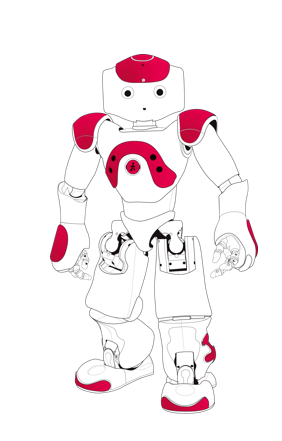
\includegraphics[scale=0.5]{nao.png}
		\caption{NAO外形}
		\label{figure 1}
	\end{figure}
    \end{columns}
\end{frame}

\begin{frame}{特点}
    \begin{itemize}
        \item 具有25个自由度
        \item 传感器遍布全身
        \item 具有2组扬声器,4组全向麦克风
        \item 官方提供丰富的SDK与开发资源
    \end{itemize}
\end{frame}

\begin{frame}{应用}
    目前NAO已被广泛应用于:
    \begin{itemize}
        \item 编程教学
        \item 科学研究
        \item 特殊教育,如NAO加入自闭症儿童的解决方案
        \item 竞技比赛
        \item 表演活动
    \end{itemize}
\end{frame}

\subsection{WHY}
\begin{frame}{背景}
    《人机物的微服务治理平台》中机器人充当连接人与物的桥梁,能否实现该平台,机器人起着至关重要的作用,姑且将NAO充当机器人的角色。
\end{frame}

\subsection{HOW}
\begin{frame}{NAO操作}
    官方提供了丰富的SDK给开发者使用,听、说、看这些暂且不谈,和本项目息息相关的有三个模块:
    \begin{itemize}
        \item ALMemory,其中ALValue getData(string key)能够获的NAO机器人的马达状态
        \item ALMotion,其中void move(float x, float y, float theta)令NAO进行移动。
        \item ALSonar,官方提供了四种检测事件,也可以从ALMemory中读取声呐数据实现自己的障碍物检测。
    \end{itemize}
\end{frame}

\subsection{路径规划}
\begin{frame}{A*算法}
    A*算法可行,但是如果栅格数量太多的话,open\ list和closed\ list将会变得很庞大,并且在路径相等的大型开放领域中搜索速度非常慢。需要改进!
\end{frame}

\begin{frame}{JPS算法}
    JPS算法就是跳点搜索算法,是对A*算法的优化。JPS算法保持了A*算法的最优性,并将搜索效率提高一个数量级甚至更多。
\end{frame}

\begin{frame}{JPS算法原理}
    未修改的A*是相当浪费的,花 了大量时间去评估一些无需评估的节点。JPS算法 能够让A*寻路更上一个档次,JPS对此是这样改进 的:识别并选择性地扩展网格地图上的仅仅某些 节点,称之为”跳点“,两个跳点连接的路径上的中间 节点将不被扩展,该方法总能计算出最优解,且能A*算法的速度提高一个数量级甚至更多。
\end{frame}

\begin{frame}{水平/垂直方向移动}
    \begin{figure}[htbp]
		\centering
		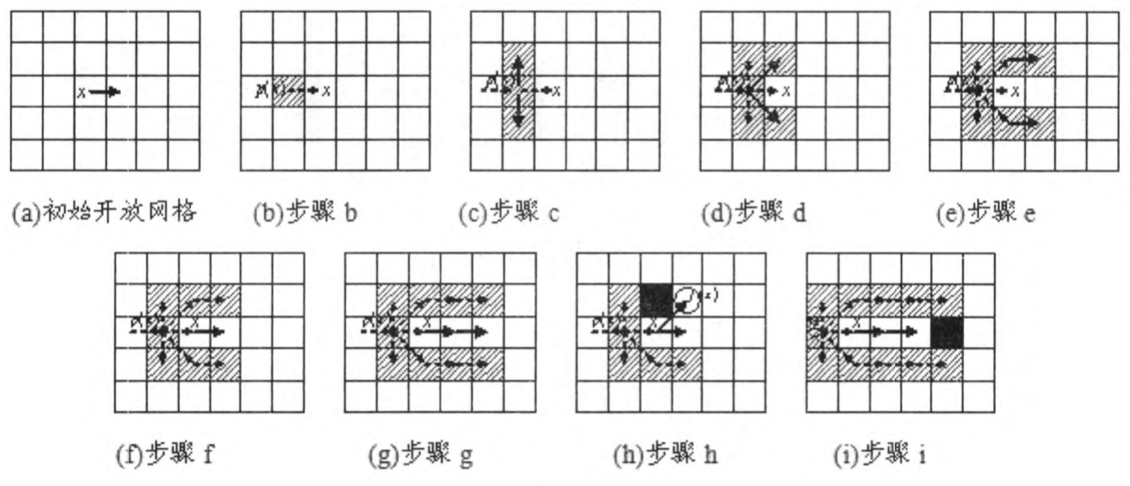
\includegraphics[scale=0.6]{figure7.png}
		\caption{水平向前移动步骤图}
		\label{figure 7}
	\end{figure}
\end{frame}

\begin{frame}{对角线方向移动}
    \begin{figure}[htbp]
		\centering
		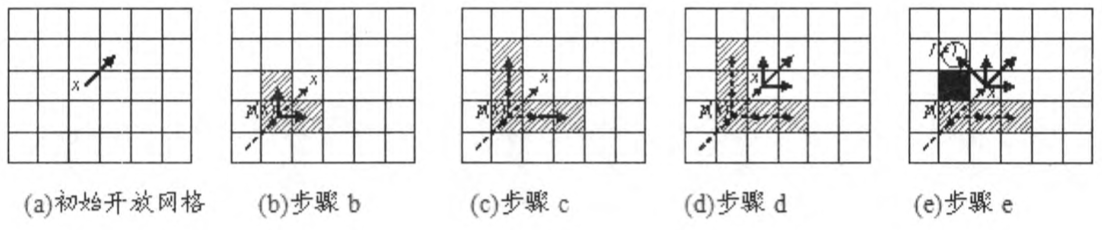
\includegraphics[scale=0.6]{figure8.png}
		\caption{对角线向前移动步骤图}
		\label{figure 8}
	\end{figure}
\end{frame}

\begin{frame}{实例}
    \begin{figure}[htbp]
		\centering
		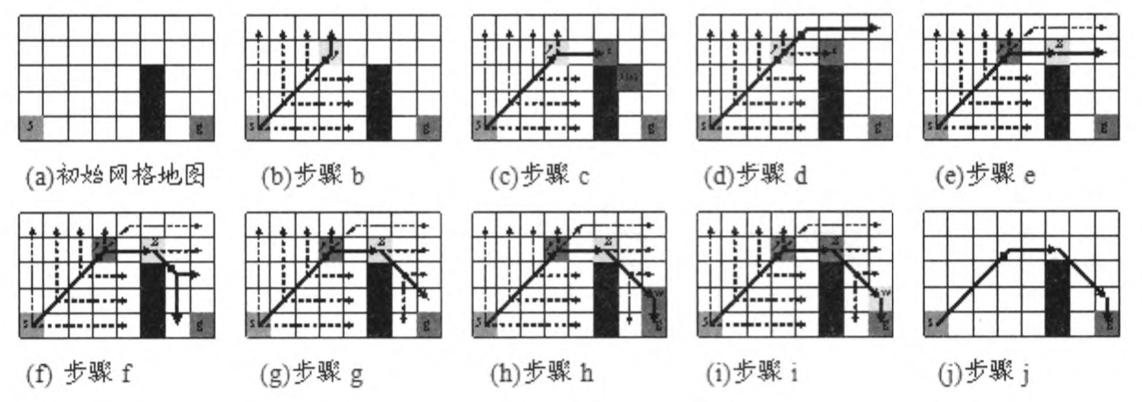
\includegraphics[scale=0.6]{figure9.png}
		\caption{算法模型实例}
		\label{figure 9}
	\end{figure}
\end{frame}

\section{数字孪生}
\subsection{WHAT}
\begin{frame}{简介}
    数 字 孪 生 (digital twin)是 以 数 字 化 方 式 创 建 物 理实体的虚拟模型,借助数据模拟物理实体在现实 环 境 中 的 行 为 ,通 过 虚 实 交 互 反 馈 、数 据 融 合 分 析 、 决策迭代优化等手段,为物理实体增加或扩展新的 能力。作为一种充分利用模型、数据、智能并集成多 学科的技术,数字孪生面向产品全生命周期过程,发 挥连接物理世界和信息世界的桥梁和纽带作用,提 供 更 加 实 时 、高 效 、智 能 的 服 务。
\end{frame}

\subsection{WHY}
\begin{frame}{意义}
    用数据模型对物理实体进行仿真、分析、决策优化等,最后物理实体可以应用优化后的决策,这样可以用最低的实际损失来获得最大的回报。
\end{frame}
\subsection{HOW}
\begin{frame}{构建数字孪生}
    有待解决
\end{frame}

\subsection{例子}
\begin{frame}{骨折复位机器人}
    \begin{columns}
    \column{0.5\textwidth}
    \begin{figure}[htbp]
		\centering
		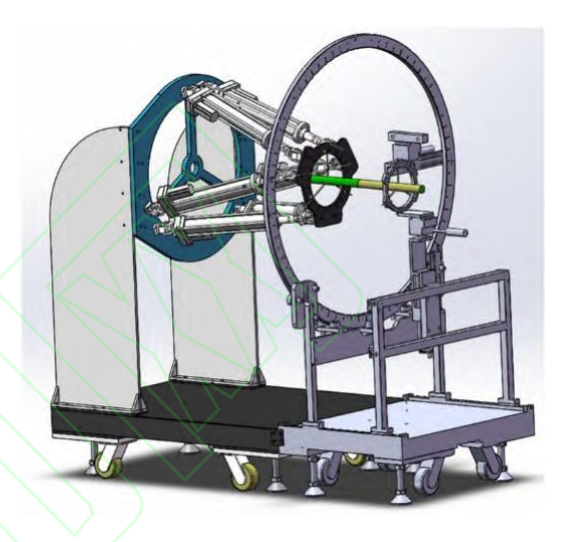
\includegraphics[scale=0.4]{figure3.png}
		\caption{骨折复位机器人实体}
		\label{figure 3}
	\end{figure}
    \column{0.5\textwidth}
	\begin{figure}[htbp]
		\centering
		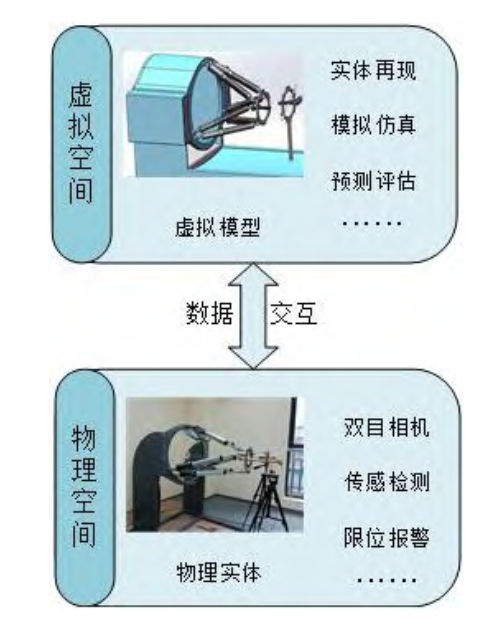
\includegraphics[scale=0.5]{figure2.png}
		\caption{数字孪生模型}
		\label{figure 2}
	\end{figure}
    \end{columns}
\end{frame}

\begin{frame}
\begin{columns}
    \column{0.5\textwidth}
    将骨折实体映射成等比例模型在测量界面进行骨折部位畸变参数的测量,确定其正位、侧位、轴位三个方向的移位和成角矫正值。
    \begin{figure}[htbp]
		\centering
		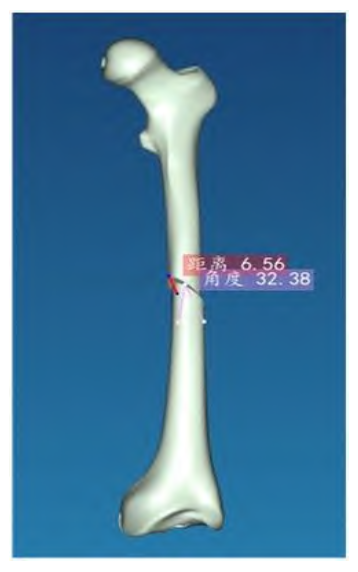
\includegraphics[scale=0.4]{figure4.png}
		\caption{骨折部位畸变值测量}
		\label{figure 4}
	\end{figure}
    \column{0.5\textwidth}
	\begin{figure}[htbp]
		\centering
		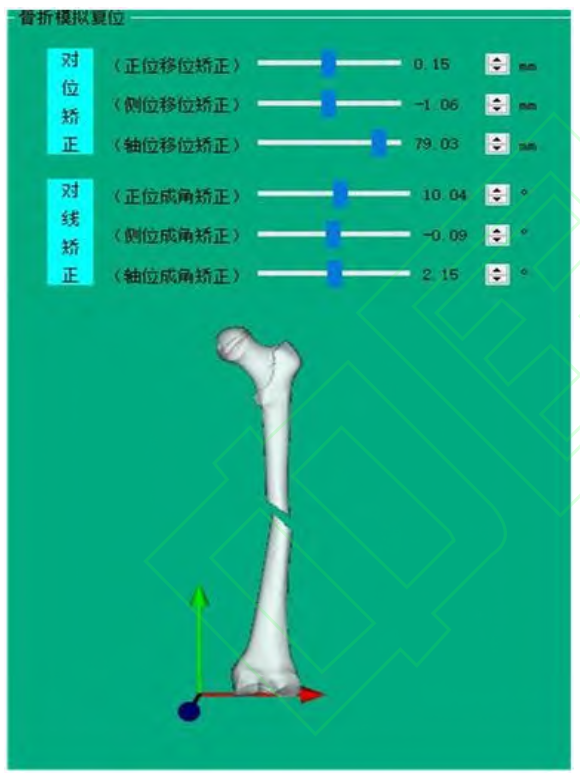
\includegraphics[scale=0.5]{figure5.png}
		\caption{骨折复位模拟矫正}
		\label{figure 5}
	\end{figure}
    \end{columns}
\end{frame}

\begin{frame}
\begin{columns}
    \column{0.5\textwidth}
    根据骨折三维模型中确定的测量值,预先进行模拟复位,先根据患者的骨 折情况对骨折部位进行三维重建,经过图像处理提取骨折复 位信息,然后将数据信息输入计算机进行计算,对复位过程 中存在的各种风险情况进行模拟比对,最终确定可行的复位 方案,然后在机器人辅助下对骨折进行复位。
    \column{0.5\textwidth}
	\begin{figure}[htbp]
		\centering
		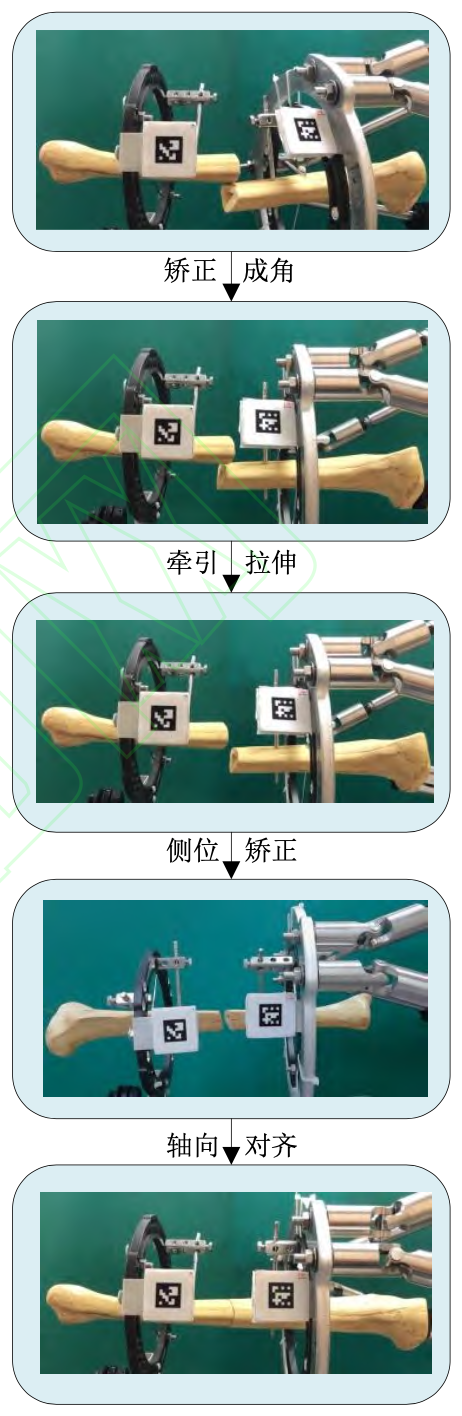
\includegraphics[scale=0.3]{figure6.png}
		\caption{机器人复位流程}
		\label{figure 6}
	\end{figure}
    \end{columns}
\end{frame}

\section{问题}
\begin{frame}{问题}
     \begin{itemize}
        \item 应用JPS算法
        \item 构建NAO数字孪生
    \end{itemize}
\end{frame}

\begin{frame}
    \centering
    Q\&A
\end{frame}
\end{document}